\refstepcounter{section}
\section*{Lecture 3: First Order Phase Transition}
\addcontentsline{toc}{section}{Lecture 3: First Order Phase Transition}
Let us now see some qualitative aspect of phase transition. Each phase transition can be viewed as a result of the failure of the stability criteria. We will see some characteristic aspects of first order phase transition\footnote{In modern language, these are called \textit{abrupt phase transition}}. However, let us first note some geometric interpretation of the thermodynamic potentials.\\[0.2cm]
We will consider the relation $G=F+PV$ which can be obtained from the Legendre transform of the internal energy. 
\begin{figure}[H]
    \centering 
    

\tikzset{every picture/.style={line width=0.75pt}} %set default line width to 0.75pt        

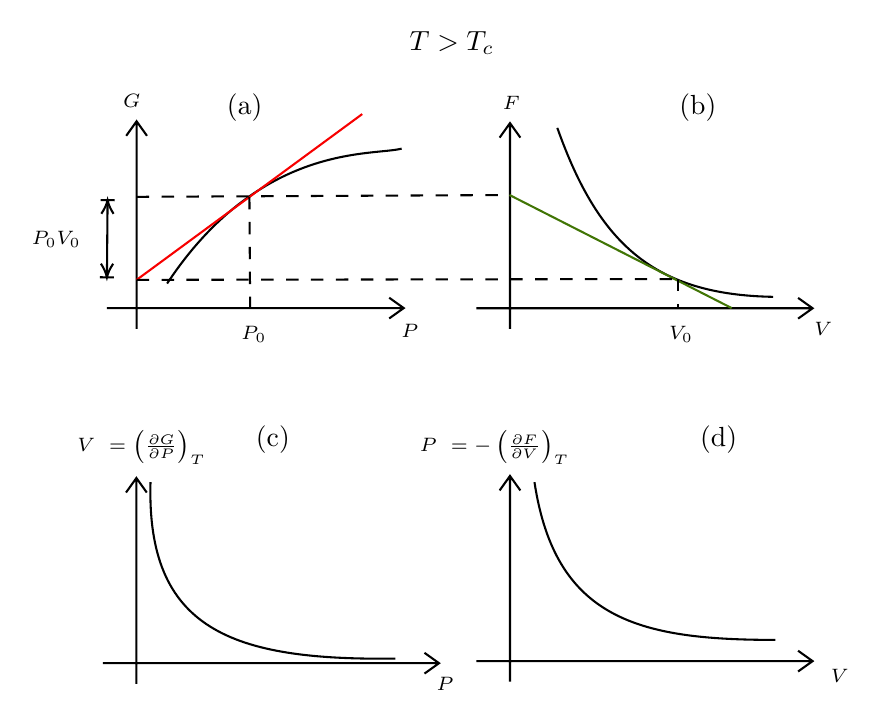
\begin{tikzpicture}[x=0.75pt,y=0.75pt,yscale=-1,xscale=1]
%uncomment if require: \path (0,381); %set diagram left start at 0, and has height of 381

%Curve Lines [id:da2867818099334498] 
\draw    (147.68,149.17) .. controls (192.68,81.17) and (246.68,87.8) .. (260.68,84.17) ;
%Curve Lines [id:da9497507659916802] 
\draw    (335.68,74.17) .. controls (355.68,130.58) and (382.68,154.58) .. (439.68,155.58) ;
%Curve Lines [id:da8862790336871029] 
\draw    (139.68,244.87) .. controls (137.68,315.87) and (178.68,330.87) .. (257.68,329.87) ;
%Curve Lines [id:da7354408741778609] 
\draw    (324.68,244.87) .. controls (334.68,310.87) and (374.68,320.87) .. (440.68,320.87) ;
%Shape: Axis 2D [id:dp08727034424643298] 
\draw  (118.68,161) -- (261.68,161)(132.98,71) -- (132.98,171) (254.68,156) -- (261.68,161) -- (254.68,166) (127.98,78) -- (132.98,71) -- (137.98,78)  ;
%Shape: Axis 2D [id:dp64041525106689] 
\draw  (296.68,161.09) -- (458.68,161.09)(312.88,71.87) -- (312.88,171) (451.68,156.09) -- (458.68,161.09) -- (451.68,166.09) (307.88,78.87) -- (312.88,71.87) -- (317.88,78.87)  ;
%Shape: Axis 2D [id:dp2378493312227148] 
\draw  (116.68,332.09) -- (278.68,332.09)(132.88,242.87) -- (132.88,342) (271.68,327.09) -- (278.68,332.09) -- (271.68,337.09) (127.88,249.87) -- (132.88,242.87) -- (137.88,249.87)  ;
%Shape: Axis 2D [id:dp9873311493222996] 
\draw  (296.68,331.09) -- (458.68,331.09)(312.88,241.87) -- (312.88,341) (451.68,326.09) -- (458.68,331.09) -- (451.68,336.09) (307.88,248.87) -- (312.88,241.87) -- (317.88,248.87)  ;
%Straight Lines [id:da5278221918963351] 
\draw [color={rgb, 255:red, 247; green, 0; blue, 0 }  ,draw opacity=1 ]   (133,147.4) -- (213.01,88.6) -- (241.68,67.53) ;
%Straight Lines [id:da9794110146885525] 
\draw [color={rgb, 255:red, 65; green, 117; blue, 5 }  ,draw opacity=1 ]   (312.68,106.53) -- (419.68,161) ;
%Straight Lines [id:da6659473404037073] 
\draw  [dash pattern={on 4.5pt off 4.5pt}]  (133,107.4) -- (312.68,106.53) ;
%Straight Lines [id:da49705295823537676] 
\draw  [dash pattern={on 4.5pt off 4.5pt}]  (133,147.4) -- (393.68,147) ;
%Straight Lines [id:da5474018860999877] 
\draw  [dash pattern={on 4.5pt off 4.5pt}]  (187.34,107.47) -- (187.68,161.28) ;
%Straight Lines [id:da7026433174042075] 
\draw  [dash pattern={on 4.5pt off 4.5pt}]  (393.68,147) -- (393.68,161) ;
%Straight Lines [id:da08583908286500619] 
\draw    (119,109) -- (118.68,146.18) ;
\draw [shift={(118.68,146.18)}, rotate = 270.49] [color={rgb, 255:red, 0; green, 0; blue, 0 }  ][line width=0.75]    (0,3.35) -- (0,-3.35)(6.56,-2.94) .. controls (4.17,-1.38) and (1.99,-0.4) .. (0,0) .. controls (1.99,0.4) and (4.17,1.38) .. (6.56,2.94)   ;
\draw [shift={(119,109)}, rotate = 90.49] [color={rgb, 255:red, 0; green, 0; blue, 0 }  ][line width=0.75]    (0,3.35) -- (0,-3.35)(6.56,-2.94) .. controls (4.17,-1.38) and (1.99,-0.4) .. (0,0) .. controls (1.99,0.4) and (4.17,1.38) .. (6.56,2.94)   ;

% Text Node
\draw (263,26.4) node [anchor=north west][inner sep=0.75pt]    {$T >T_{c}$};
% Text Node
\draw (125,56.4) node [anchor=north west][inner sep=0.75pt]  [font=\scriptsize]  {$G$};
% Text Node
\draw (259,167.4) node [anchor=north west][inner sep=0.75pt]  [font=\scriptsize]  {$P$};
% Text Node
\draw (276,337.4) node [anchor=north west][inner sep=0.75pt]  [font=\scriptsize]  {$P$};
% Text Node
\draw (466,333.4) node [anchor=north west][inner sep=0.75pt]  [font=\scriptsize]  {$V$};
% Text Node
\draw (458,166.4) node [anchor=north west][inner sep=0.75pt]  [font=\scriptsize]  {$V$};
% Text Node
\draw (268,218.4) node [anchor=north west][inner sep=0.75pt]  [font=\scriptsize]  {$P\ =-\left(\frac{\partial F}{\partial V}\right)_{T} \ $};
% Text Node
\draw (103,218.4) node [anchor=north west][inner sep=0.75pt]  [font=\scriptsize]  {$V\ =\left(\frac{\partial G}{\partial P}\right)_{T}$};
% Text Node
\draw (308,57.4) node [anchor=north west][inner sep=0.75pt]  [font=\scriptsize]  {$F$};
% Text Node
\draw (81,122.4) node [anchor=north west][inner sep=0.75pt]  [font=\scriptsize]  {$P_{0} V_{0}$};
% Text Node
\draw (388,168.4) node [anchor=north west][inner sep=0.75pt]  [font=\scriptsize]  {$V_{0}$};
% Text Node
\draw (182,168.4) node [anchor=north west][inner sep=0.75pt]  [font=\scriptsize]  {$P_{0}$};
% Text Node
\draw (175,56) node [anchor=north west][inner sep=0.75pt]   [align=left] {(a)};
% Text Node
\draw (393,56) node [anchor=north west][inner sep=0.75pt]   [align=left] {(b)};
% Text Node
\draw (189,216) node [anchor=north west][inner sep=0.75pt]   [align=left] {(c)};
% Text Node
\draw (403,216) node [anchor=north west][inner sep=0.75pt]   [align=left] {(d)};


\end{tikzpicture}

    \caption{\textbf{Relation between $\mathbf{G}$ and $\mathbf{F}$.} (a) Variation of Gibbs potential with pressure at a temperature $T>T_c$ (b) Corresponding plot of Helmholtz potential with $V$ (c) and (d) denotes the P-V diagrams constructed from these potentials}
    \label{fig:lec31}
\end{figure}
\noindent
In the above figure, observe the plot of $G$ vs. $P$, which is smooth. We draw the tangent line at a $P=P_0$ and this intercepts the y-axis somewhere. The equation of the tangent is $G= PV+c$ as $V = \qty(\pdv{G}{P})_{T,N}$ and it passes through the point $(P_0, G_0)$. Thus we have,
$$G_0 = P_0 V_0 + c \implies c = G_0-P_0V_0$$
The tangent has an intercept of $G_0-P_0V_0$ and so the remaining length as shown by the arrow in is Fig.\ref{fig:lec31} (a) is $G_0-(G_0-P_0V_0) = P_0V_0$. From the length of the intercept of the tangent, we can obtain the Helmholtz potential for this value of $P_0$. We also obtain the volume from the slope of the tangent. The corresponding $F$ vs. $V$ graph has been plotted using these values. Also, plotted are the $V$ vs. $P$ graph (using the slope of the tangent of the Gibbs potential) and the $P$ vs. $V$ graph (using the slope of the tangent of the Helmholtz potential ). This is the case for $T>T_c$. Now let us see the case when $T<T_c$ and the phase transition has occurred. We will see this with respect to the Van der Waal's equation.
\begin{figure}[H]
    \centering
    

\tikzset{every picture/.style={line width=0.75pt}} %set default line width to 0.75pt        

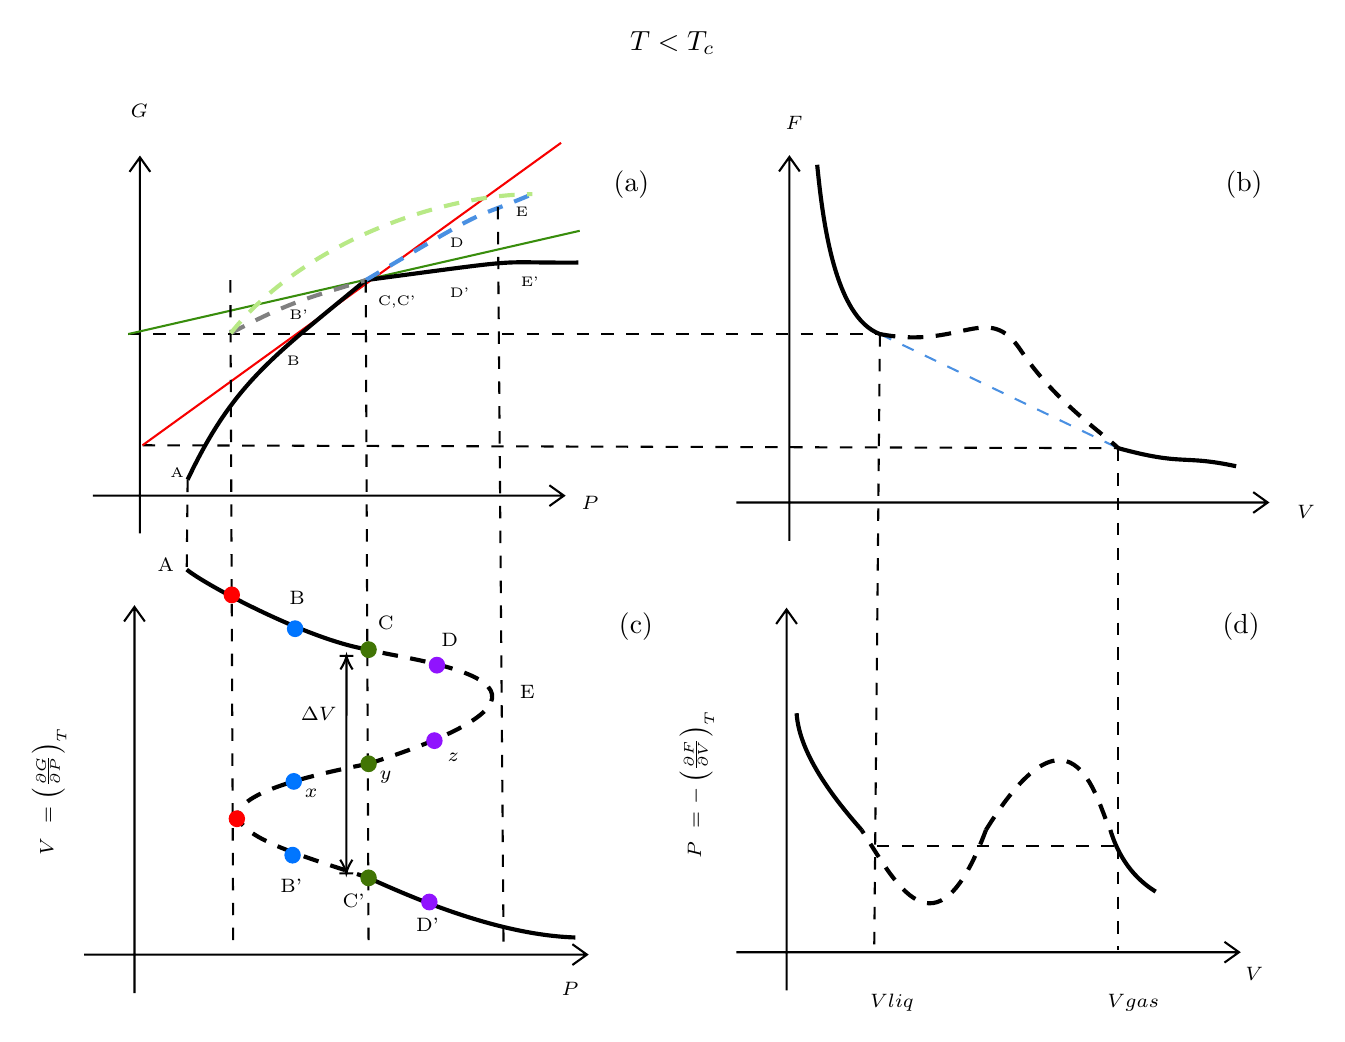
\begin{tikzpicture}[x=0.75pt,y=0.75pt,yscale=-1,xscale=1]
%uncomment if require: \path (0,590); %set diagram left start at 0, and has height of 590

%Shape: Axis 2D [id:dp4775489840555638] 
\draw  (59.34,263.8) -- (286.32,263.8)(82.04,100.79) -- (82.04,281.92) (279.32,258.8) -- (286.32,263.8) -- (279.32,268.8) (77.04,107.79) -- (82.04,100.79) -- (87.04,107.79)  ;
%Shape: Axis 2D [id:dp42588900332731494] 
\draw  (55.19,484.92) -- (297.4,484.92)(79.41,317.42) -- (79.41,503.53) (290.4,479.92) -- (297.4,484.92) -- (290.4,489.92) (74.41,324.42) -- (79.41,317.42) -- (84.41,324.42)  ;
%Shape: Axis 2D [id:dp9600862518493296] 
\draw  (369.36,483.77) -- (611.57,483.77)(393.59,318.62) -- (393.59,502.12) (604.57,478.77) -- (611.57,483.77) -- (604.57,488.77) (388.59,325.62) -- (393.59,318.62) -- (398.59,325.62)  ;
%Straight Lines [id:da06664426102620935] 
\draw  [dash pattern={on 4.5pt off 4.5pt}]  (76.39,185.95) -- (438.57,185.95) ;
%Shape: Axis 2D [id:dp021821544978374297] 
\draw  (369.36,267.1) -- (625.41,267.1)(394.97,100.6) -- (394.97,285.61) (618.41,262.1) -- (625.41,267.1) -- (618.41,272.1) (389.97,107.6) -- (394.97,100.6) -- (399.97,107.6)  ;
%Straight Lines [id:da2713236341625831] 
\draw  [dash pattern={on 4.5pt off 4.5pt}]  (83.31,239.52) -- (553.44,240.93) ;
%Straight Lines [id:da4024260343011937] 
\draw [color={rgb, 255:red, 74; green, 144; blue, 226 }  ,draw opacity=1 ] [dash pattern={on 4.5pt off 4.5pt}]  (438.57,185.95) -- (553.44,240.93) ;
%Straight Lines [id:da00607710951650009] 
\draw [color={rgb, 255:red, 247; green, 0; blue, 0 }  ,draw opacity=1 ]   (83.31,239.52) -- (284.94,93.81) ;
%Straight Lines [id:da3169244653349518] 
\draw [color={rgb, 255:red, 56; green, 141; blue, 12 }  ,draw opacity=1 ]   (76.39,185.95) -- (293.94,136.19) ;
%Curve Lines [id:da4120975232185071] 
\draw [line width=1.5]    (105.02,256.11) .. controls (127.16,209.31) and (146.54,196.62) .. (190.83,159.96) ;
%Curve Lines [id:da5676309808224264] 
\draw [line width=1.5]    (190.83,159.96) .. controls (273.87,148.94) and (248.95,151.76) .. (293.24,151.5) ;
%Curve Lines [id:da8621306379129015] 
\draw [color={rgb, 255:red, 74; green, 144; blue, 226 }  ,draw opacity=1 ][line width=1.5]  [dash pattern={on 5.63pt off 4.5pt}]  (190.83,159.96) .. controls (255.87,121.35) and (237.88,132.63) .. (271.1,118.53) ;
%Curve Lines [id:da36758197229500567] 
\draw [color={rgb, 255:red, 128; green, 128; blue, 128 }  ,draw opacity=1 ][line width=1.5]  [dash pattern={on 5.63pt off 4.5pt}]  (125.78,185.53) .. controls (154.84,170.02) and (163.15,168.61) .. (190.83,159.96) ;
%Straight Lines [id:da567228132201586] 
\draw  [dash pattern={on 4.5pt off 4.5pt}]  (190.83,159.96) -- (192.21,482.87) ;
%Straight Lines [id:da9483033768768598] 
\draw  [dash pattern={on 4.5pt off 4.5pt}]  (438.57,185.95) -- (435.8,484.28) ;
%Straight Lines [id:da9217488527545249] 
\draw  [dash pattern={on 4.5pt off 4.5pt}]  (553.44,240.93) -- (553.44,482.87) ;
%Straight Lines [id:da2854862917140152] 
\draw  [dash pattern={on 4.5pt off 4.5pt}]  (125.61,159.96) -- (127,482.87) ;
%Straight Lines [id:da07961783889145901] 
\draw  [dash pattern={on 4.5pt off 4.5pt}]  (254.49,124.71) -- (257.26,483.16) ;
%Straight Lines [id:da7053384608200847] 
\draw  [dash pattern={on 4.5pt off 4.5pt}]  (437.18,432.45) -- (553.44,432.45) ;
%Curve Lines [id:da5085181279509152] 
\draw [line width=1.5]  [dash pattern={on 5.63pt off 4.5pt}]  (438.57,185.95) .. controls (478.07,193.61) and (490.5,169.77) .. (506.51,193.9) .. controls (522.52,218.03) and (545.79,233.67) .. (553.44,240.93) ;
%Curve Lines [id:da9700091203275132] 
\draw [line width=1.5]    (553.44,240.93) .. controls (585.27,249.63) and (583.89,243.99) .. (610.18,249.63) ;
%Curve Lines [id:da6521675384951386] 
\draw [line width=1.5]    (438.57,185.95) .. controls (416.42,177.72) and (410.89,129.79) .. (408.34,104.4) ;
%Curve Lines [id:da8871946832735184] 
\draw [line width=1.5]    (291.86,476.67) .. controls (254.49,475.52) and (212.97,457.38) .. (192.21,447.96) ;
%Curve Lines [id:da9310543436543585] 
\draw [line width=1.5]    (192.21,337.98) .. controls (163.15,333.45) and (112.9,306.45) .. (104.59,299.4) ;
%Curve Lines [id:da009950191800251806] 
\draw [line width=1.5]  [dash pattern={on 5.63pt off 4.5pt}]  (192.21,392.97) .. controls (316.77,353.19) and (210.2,343.32) .. (192.21,337.98) ;
%Curve Lines [id:da5014976599202591] 
\draw [line width=1.5]  [dash pattern={on 5.63pt off 4.5pt}]  (192.21,392.97) .. controls (177.19,395.88) and (165.33,398.71) .. (156.17,401.47) .. controls (94.4,420.06) and (154.85,435.29) .. (192.21,447.96) ;
%Curve Lines [id:da2665685827610216] 
\draw [line width=1.5]    (398.43,368.63) .. controls (399.68,389.72) and (419.46,413.16) .. (429.73,424.87) ;
%Curve Lines [id:da7879739467019476] 
\draw [line width=1.5]    (549.59,424.87) .. controls (554.53,441.28) and (563.75,449.87) .. (571.43,454.56) ;
%Curve Lines [id:da6255359832443886] 
\draw [line width=1.5]  [dash pattern={on 5.63pt off 4.5pt}]  (489.66,424.87) .. controls (533.02,354.56) and (543.77,414.72) .. (549.59,424.87) ;
%Curve Lines [id:da5195232035004981] 
\draw [line width=1.5]  [dash pattern={on 5.63pt off 4.5pt}]  (489.66,424.87) .. controls (465.12,490.5) and (445.58,449.09) .. (429.73,424.87) ;
%Curve Lines [id:da39801638316834276] 
\draw [color={rgb, 255:red, 184; green, 233; blue, 134 }  ,draw opacity=1 ][line width=1.5]  [dash pattern={on 5.63pt off 4.5pt}]  (125.78,185.53) .. controls (160.38,142.01) and (226.81,118.79) .. (271.1,118.53) ;
%Straight Lines [id:da8192124936289387] 
\draw    (181.58,340.97) -- (181.47,445.79) ;
\draw [shift={(181.47,445.79)}, rotate = 270.06] [color={rgb, 255:red, 0; green, 0; blue, 0 }  ][line width=0.75]    (0,3.35) -- (0,-3.35)(6.56,-2.94) .. controls (4.17,-1.38) and (1.99,-0.4) .. (0,0) .. controls (1.99,0.4) and (4.17,1.38) .. (6.56,2.94)   ;
\draw [shift={(181.58,340.97)}, rotate = 90.06] [color={rgb, 255:red, 0; green, 0; blue, 0 }  ][line width=0.75]    (0,3.35) -- (0,-3.35)(6.56,-2.94) .. controls (4.17,-1.38) and (1.99,-0.4) .. (0,0) .. controls (1.99,0.4) and (4.17,1.38) .. (6.56,2.94)   ;
%Straight Lines [id:da9228370233494249] 
\draw  [dash pattern={on 4.5pt off 4.5pt}]  (105.02,256.11) -- (104.59,299.4) ;
%Shape: Ellipse [id:dp7896549563334632] 
\draw  [color={rgb, 255:red, 255; green, 0; blue, 0 }  ,draw opacity=1 ][fill={rgb, 255:red, 255; green, 0; blue, 0 }  ,fill opacity=1 ] (122.86,311.6) .. controls (122.86,309.65) and (124.4,308.06) .. (126.3,308.06) .. controls (128.21,308.06) and (129.75,309.65) .. (129.75,311.6) .. controls (129.75,313.56) and (128.21,315.15) .. (126.3,315.15) .. controls (124.4,315.15) and (122.86,313.56) .. (122.86,311.6) -- cycle ;
%Shape: Ellipse [id:dp35529400630968067] 
\draw  [color={rgb, 255:red, 255; green, 0; blue, 0 }  ,draw opacity=1 ][fill={rgb, 255:red, 255; green, 0; blue, 0 }  ,fill opacity=1 ] (125.3,419.45) .. controls (125.3,417.5) and (126.84,415.91) .. (128.75,415.91) .. controls (130.65,415.91) and (132.19,417.5) .. (132.19,419.45) .. controls (132.19,421.41) and (130.65,423) .. (128.75,423) .. controls (126.84,423) and (125.3,421.41) .. (125.3,419.45) -- cycle ;
%Shape: Ellipse [id:dp4590266716443322] 
\draw  [color={rgb, 255:red, 0; green, 115; blue, 255 }  ,draw opacity=1 ][fill={rgb, 255:red, 0; green, 118; blue, 255 }  ,fill opacity=1 ] (153.36,327.91) .. controls (153.36,325.95) and (154.91,324.36) .. (156.81,324.36) .. controls (158.71,324.36) and (160.26,325.95) .. (160.26,327.91) .. controls (160.26,329.86) and (158.71,331.45) .. (156.81,331.45) .. controls (154.91,331.45) and (153.36,329.86) .. (153.36,327.91) -- cycle ;
%Shape: Ellipse [id:dp4904216040989311] 
\draw  [color={rgb, 255:red, 0; green, 115; blue, 255 }  ,draw opacity=1 ][fill={rgb, 255:red, 0; green, 118; blue, 255 }  ,fill opacity=1 ] (152.72,401.47) .. controls (152.72,399.51) and (154.26,397.93) .. (156.17,397.93) .. controls (158.07,397.93) and (159.62,399.51) .. (159.62,401.47) .. controls (159.62,403.42) and (158.07,405.01) .. (156.17,405.01) .. controls (154.26,405.01) and (152.72,403.42) .. (152.72,401.47) -- cycle ;
%Shape: Ellipse [id:dp5041954985396434] 
\draw  [color={rgb, 255:red, 0; green, 115; blue, 255 }  ,draw opacity=1 ][fill={rgb, 255:red, 0; green, 118; blue, 255 }  ,fill opacity=1 ] (152.14,437.01) .. controls (152.14,435.05) and (153.69,433.47) .. (155.59,433.47) .. controls (157.49,433.47) and (159.04,435.05) .. (159.04,437.01) .. controls (159.04,438.97) and (157.49,440.55) .. (155.59,440.55) .. controls (153.69,440.55) and (152.14,438.97) .. (152.14,437.01) -- cycle ;
%Shape: Ellipse [id:dp7815464804668679] 
\draw  [color={rgb, 255:red, 65; green, 117; blue, 5 }  ,draw opacity=1 ][fill={rgb, 255:red, 65; green, 117; blue, 5 }  ,fill opacity=1 ] (188.76,337.98) .. controls (188.76,336.03) and (190.31,334.44) .. (192.21,334.44) .. controls (194.11,334.44) and (195.66,336.03) .. (195.66,337.98) .. controls (195.66,339.94) and (194.11,341.53) .. (192.21,341.53) .. controls (190.31,341.53) and (188.76,339.94) .. (188.76,337.98) -- cycle ;
%Shape: Ellipse [id:dp7343848852090362] 
\draw  [color={rgb, 255:red, 65; green, 117; blue, 5 }  ,draw opacity=1 ][fill={rgb, 255:red, 65; green, 117; blue, 5 }  ,fill opacity=1 ] (188.76,392.97) .. controls (188.76,391.01) and (190.31,389.43) .. (192.21,389.43) .. controls (194.11,389.43) and (195.66,391.01) .. (195.66,392.97) .. controls (195.66,394.93) and (194.11,396.51) .. (192.21,396.51) .. controls (190.31,396.51) and (188.76,394.93) .. (188.76,392.97) -- cycle ;
%Shape: Ellipse [id:dp9387347836897418] 
\draw  [color={rgb, 255:red, 65; green, 117; blue, 5 }  ,draw opacity=1 ][fill={rgb, 255:red, 65; green, 117; blue, 5 }  ,fill opacity=1 ] (188.76,447.96) .. controls (188.76,446) and (190.31,444.41) .. (192.21,444.41) .. controls (194.11,444.41) and (195.66,446) .. (195.66,447.96) .. controls (195.66,449.91) and (194.11,451.5) .. (192.21,451.5) .. controls (190.31,451.5) and (188.76,449.91) .. (188.76,447.96) -- cycle ;
%Shape: Ellipse [id:dp057556742753685386] 
\draw  [color={rgb, 255:red, 144; green, 19; blue, 254 }  ,draw opacity=1 ][fill={rgb, 255:red, 144; green, 19; blue, 254 }  ,fill opacity=1 ] (221.7,345.46) .. controls (221.7,343.51) and (223.24,341.92) .. (225.14,341.92) .. controls (227.05,341.92) and (228.59,343.51) .. (228.59,345.46) .. controls (228.59,347.42) and (227.05,349.01) .. (225.14,349.01) .. controls (223.24,349.01) and (221.7,347.42) .. (221.7,345.46) -- cycle ;
%Shape: Ellipse [id:dp30607195698011547] 
\draw  [color={rgb, 255:red, 144; green, 19; blue, 254 }  ,draw opacity=1 ][fill={rgb, 255:red, 144; green, 19; blue, 254 }  ,fill opacity=1 ] (220.48,381.83) .. controls (220.48,379.87) and (222.02,378.29) .. (223.92,378.29) .. controls (225.83,378.29) and (227.37,379.87) .. (227.37,381.83) .. controls (227.37,383.79) and (225.83,385.37) .. (223.92,385.37) .. controls (222.02,385.37) and (220.48,383.79) .. (220.48,381.83) -- cycle ;
%Shape: Ellipse [id:dp1148942836940231] 
\draw  [color={rgb, 255:red, 144; green, 19; blue, 254 }  ,draw opacity=1 ][fill={rgb, 255:red, 144; green, 19; blue, 254 }  ,fill opacity=1 ] (218.03,459.58) .. controls (218.03,457.63) and (219.58,456.04) .. (221.48,456.04) .. controls (223.39,456.04) and (224.93,457.63) .. (224.93,459.58) .. controls (224.93,461.54) and (223.39,463.12) .. (221.48,463.12) .. controls (219.58,463.12) and (218.03,461.54) .. (218.03,459.58) -- cycle ;

% Text Node
\draw (316.74,38.83) node [anchor=north west][inner sep=0.75pt]    {$T< T_{c}$};
% Text Node
\draw (76.12,73.84) node [anchor=north west][inner sep=0.75pt]  [font=\scriptsize]  {$G$};
% Text Node
\draw (293.41,262.76) node [anchor=north west][inner sep=0.75pt]  [font=\scriptsize]  {$P$};
% Text Node
\draw (283.72,496.81) node [anchor=north west][inner sep=0.75pt]  [font=\scriptsize]  {$P$};
% Text Node
\draw (613.12,489.76) node [anchor=north west][inner sep=0.75pt]  [font=\scriptsize]  {$V$};
% Text Node
\draw (638.03,266.99) node [anchor=north west][inner sep=0.75pt]  [font=\scriptsize]  {$V$};
% Text Node
\draw (340.55,440.33) node [anchor=north west][inner sep=0.75pt]  [font=\scriptsize,rotate=-270]  {$P\ =-\left(\frac{\partial F}{\partial V}\right)_{T} \ $};
% Text Node
\draw (28.46,438.44) node [anchor=north west][inner sep=0.75pt]  [font=\scriptsize,rotate=-270]  {$V\ =\left(\frac{\partial G}{\partial P}\right)_{T}$};
% Text Node
\draw (391.68,79.48) node [anchor=north west][inner sep=0.75pt]  [font=\scriptsize]  {$F$};
% Text Node
\draw (158.05,364.43) node [anchor=north west][inner sep=0.75pt]  [font=\scriptsize]  {$\Delta V$};
% Text Node
\draw (308.79,105.68) node [anchor=north west][inner sep=0.75pt]   [align=left] {(a)};
% Text Node
\draw (603.58,105.68) node [anchor=north west][inner sep=0.75pt]   [align=left] {(b)};
% Text Node
\draw (311.36,318.58) node [anchor=north west][inner sep=0.75pt]   [align=left] {(c)};
% Text Node
\draw (602.2,318.58) node [anchor=north west][inner sep=0.75pt]   [align=left] {(d)};
% Text Node
\draw (432.35,502.45) node [anchor=north west][inner sep=0.75pt]  [font=\scriptsize]  {$V\tund{liq}$};
% Text Node
\draw (546.61,502.68) node [anchor=north west][inner sep=0.75pt]  [font=\scriptsize]  {$V\tund{gas}$};
% Text Node
\draw (89.11,292.23) node [anchor=north west][inner sep=0.75pt]  [font=\scriptsize] [align=left] {A};
% Text Node
\draw (152.56,308.53) node [anchor=north west][inner sep=0.75pt]  [font=\scriptsize] [align=left] {B};
% Text Node
\draw (148.27,446.85) node [anchor=north west][inner sep=0.75pt]  [font=\scriptsize] [align=left] {B'};
% Text Node
\draw (195.17,320.31) node [anchor=north west][inner sep=0.75pt]  [font=\scriptsize] [align=left] {C};
% Text Node
\draw (225.77,328.6) node [anchor=north west][inner sep=0.75pt]  [font=\scriptsize] [align=left] {D};
% Text Node
\draw (160.04,403.49) node [anchor=north west][inner sep=0.75pt]  [font=\scriptsize]  {$x$};
% Text Node
\draw (196.08,394.99) node [anchor=north west][inner sep=0.75pt]  [font=\scriptsize]  {$y$};
% Text Node
\draw (263.6,353.68) node [anchor=north west][inner sep=0.75pt]  [font=\scriptsize] [align=left] {E};
% Text Node
\draw (178.2,454.49) node [anchor=north west][inner sep=0.75pt]  [font=\scriptsize] [align=left] {C'};
% Text Node
\draw (213.58,465.78) node [anchor=north west][inner sep=0.75pt]  [font=\scriptsize] [align=left] {D'};
% Text Node
\draw (151.34,195.16) node [anchor=north west][inner sep=0.75pt]  [font=\tiny] [align=left] {B};
% Text Node
\draw (95.21,249.08) node [anchor=north west][inner sep=0.75pt]  [font=\tiny] [align=left] {A};
% Text Node
\draw (195.14,165.86) node [anchor=north west][inner sep=0.75pt]  [font=\tiny] [align=left] {C,C'};
% Text Node
\draw (229.86,138.27) node [anchor=north west][inner sep=0.75pt]  [font=\tiny] [align=left] {D};
% Text Node
\draw (261.59,123.23) node [anchor=north west][inner sep=0.75pt]  [font=\tiny] [align=left] {E};
% Text Node
\draw (228.8,386.14) node [anchor=north west][inner sep=0.75pt]  [font=\scriptsize]  {$z$};
% Text Node
\draw (229.86,162.1) node [anchor=north west][inner sep=0.75pt]  [font=\tiny] [align=left] {D'};
% Text Node
\draw (264.03,157.09) node [anchor=north west][inner sep=0.75pt]  [font=\tiny] [align=left] {E'};
% Text Node
\draw (152.56,172.59) node [anchor=north west][inner sep=0.75pt]  [font=\tiny] [align=left] {B'};
\end{tikzpicture}

    \caption{Plot of different quantities for $T<T_c$}
    \label{fig:lec32}
\end{figure}
\noindent
In this scenario, $G$ will have a `kink' for some pressure $P=P_0$, since for first order phase transition, the derivative of the free energy is discontinuous. At this point, $\qty(\pdv[2]{G}{P}) \to \infty$ (even though this quantity cannot be defined exactly at $P=P_0$) and using Eq.\eqref{eqn:inverseGA}, we get $\qty(\pdv{A}{V})=0$. Thus we expect that the corresponding plot of $A$ has a \textit{straight line} portion, as is shown in Fig.\ref{fig:lec32} (b) with a blue dashed line.\\[0.2cm]
Let us now see how the plot of $G$ in (a) is actually constructed. For that, we need the isotherm in (c). Let us start at $A$ and then, integrating we have $$G(P)-G(P\tund{A}) = \int\limits_{P\tund{A}}^{P}V\dd P$$ and we do this for all values of $P$. This creates a closed loop kind of plot, since for a single $P$, we have three values of $V$. Note that, this disappears for higher temperature since then, Van der Waal's equation consists of only one real and two complex roots. \\[0.2cm]
What happens physically? Let us suppose our system is in a temperature bath and the temperature is fixed. So, consider the isotherm in (c) and start increasing pressure from $P_A$. The system will follow this isotherm. At $P_A$, there is a unique volume and thus a unique state of the system. Now, if we increase further, for each pressure, we will get multiple values of volume, so there are different states to choose from.\\[0.2cm] Consider the blue points (all having same $P$ but different $V$). Of these, the state $x$ is unstable and hence the system has two states B and B' to choose from. The state chosen is the one with the minimum value of $G$ which is determined from panel (a). As clearly seen, the physical state chosen is B. Increasing pressure further, we get to C where the kink is there.\\[0.2cm] On increasing further, we see that the state chosen is $D'$ since this has lesser value of $G$. The blue and gray dashed lines in (a) denote the branch of $G$ with higher value of $G$ and thus, is not chosen. The green dashed line represent the unstable region where the states, say $x,y$ or $z$ lies. We see that in (c), no state from the dashed region is selected and hence after $C$, there is a volume jump, denoted by $\Delta V$. The physical isotherm is thus the one created from the Maxwell equal area construction (as discussed before). \\[0.2cm]
The points C and C' are determined by the condition that $G(P_c) = G(P_{c'})$ and hence, $\int\limits_{P_c}^{P_{c'}}V\dd P = 0$, which proves that the areas divided by the line segment are indeed equal.\\[0.5cm]
\begin{figure}[H]
\centering 


\tikzset{every picture/.style={line width=0.75pt}} %set default line width to 0.75pt        

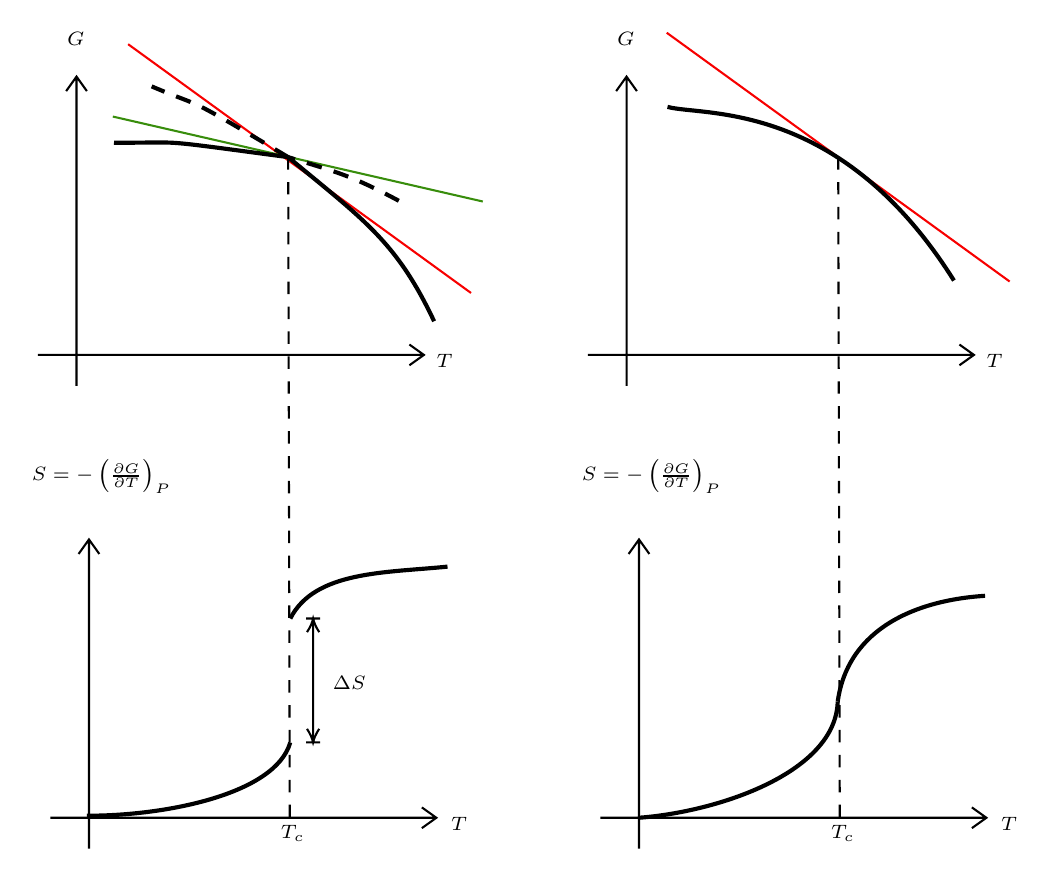
\begin{tikzpicture}[x=0.75pt,y=0.75pt,yscale=-1,xscale=1]
%uncomment if require: \path (0,590); %set diagram left start at 0, and has height of 590

%Shape: Axis 2D [id:dp8981725818269322] 
\draw  (59.34,229.67) -- (245.32,229.67)(77.94,95.58) -- (77.94,244.57) (238.32,224.67) -- (245.32,229.67) -- (238.32,234.67) (72.94,102.58) -- (77.94,95.58) -- (82.94,102.58)  ;
%Straight Lines [id:da10289878744307912] 
\draw [color={rgb, 255:red, 247; green, 0; blue, 0 }  ,draw opacity=1 ]   (268.01,199.83) -- (102.8,79.97) ;
%Straight Lines [id:da2258871588445236] 
\draw [color={rgb, 255:red, 56; green, 141; blue, 12 }  ,draw opacity=1 ]   (273.68,155.76) -- (95.43,114.83) ;
%Curve Lines [id:da9615091055645277] 
\draw [line width=1.5]    (250.23,213.47) .. controls (232.08,174.97) and (216.21,164.53) .. (179.92,134.38) ;
%Curve Lines [id:da8359707620668627] 
\draw [line width=1.5]    (179.92,134.38) .. controls (111.88,125.31) and (132.29,127.63) .. (96,127.42) ;
%Curve Lines [id:da8340943114953978] 
\draw [color={rgb, 255:red, 0; green, 0; blue, 0 }  ,draw opacity=1 ][line width=1.5]  [dash pattern={on 5.63pt off 4.5pt}]  (179.92,134.38) .. controls (126.62,102.62) and (141.36,111.9) .. (114.15,100.3) ;
%Curve Lines [id:da96995686150974] 
\draw [color={rgb, 255:red, 0; green, 0; blue, 0 }  ,draw opacity=1 ][line width=1.5]  [dash pattern={on 5.63pt off 4.5pt}]  (233.22,155.41) .. controls (209.4,142.65) and (202.6,141.49) .. (179.92,134.38) ;
%Shape: Axis 2D [id:dp8554302905464903] 
\draw  (65.34,452.67) -- (251.32,452.67)(83.94,318.58) -- (83.94,467.57) (244.32,447.67) -- (251.32,452.67) -- (244.32,457.67) (78.94,325.58) -- (83.94,318.58) -- (88.94,325.58)  ;
%Curve Lines [id:da12282513426344555] 
\draw [line width=1.5]    (180.92,416.38) .. controls (173.68,441.78) and (119.23,451.88) .. (82.94,451.67) ;
%Straight Lines [id:da38473547163246413] 
\draw  [dash pattern={on 4.5pt off 4.5pt}]  (179.92,134.38) -- (180.68,453.08) ;
%Curve Lines [id:da93212726343251] 
\draw [line width=1.5]    (256.68,331.68) .. controls (226.68,334.68) and (192.68,333.68) .. (180.94,356.67) ;
%Shape: Axis 2D [id:dp7665792369835268] 
\draw  (324.34,229.67) -- (510.32,229.67)(342.94,95.58) -- (342.94,244.57) (503.32,224.67) -- (510.32,229.67) -- (503.32,234.67) (337.94,102.58) -- (342.94,95.58) -- (347.94,102.58)  ;
%Straight Lines [id:da8952029366933306] 
\draw [color={rgb, 255:red, 247; green, 0; blue, 0 }  ,draw opacity=1 ]   (527.52,194.31) -- (362.31,74.45) ;
%Shape: Axis 2D [id:dp4609745890865987] 
\draw  (330.34,452.67) -- (516.32,452.67)(348.94,318.58) -- (348.94,467.57) (509.32,447.67) -- (516.32,452.67) -- (509.32,457.67) (343.94,325.58) -- (348.94,318.58) -- (353.94,325.58)  ;
%Curve Lines [id:da21371653241026622] 
\draw [line width=1.5]    (444.68,396.73) .. controls (443.68,430.73) and (387.68,449.73) .. (348.94,452.67) ;
%Straight Lines [id:da6172230050075982] 
\draw  [dash pattern={on 4.5pt off 4.5pt}]  (444.92,134.38) -- (445.68,453.08) ;
%Curve Lines [id:da6934067336868084] 
\draw [line width=1.5]    (515.68,345.73) .. controls (483.68,347.73) and (449.68,360.73) .. (444.68,396.73) ;
%Shape: Boxed Bezier Curve [id:dp45110897311934406] 
\draw [line width=1.5]    (500.68,193.83) .. controls (445.73,106.31) and (379.78,114.84) .. (362.68,110.17) ;
%Straight Lines [id:da29524891858438607] 
\draw    (191.94,356.67) -- (191.92,416.38) ;
\draw [shift={(191.92,416.38)}, rotate = 270.02] [color={rgb, 255:red, 0; green, 0; blue, 0 }  ][line width=0.75]    (0,3.35) -- (0,-3.35)(6.56,-2.94) .. controls (4.17,-1.38) and (1.99,-0.4) .. (0,0) .. controls (1.99,0.4) and (4.17,1.38) .. (6.56,2.94)   ;
\draw [shift={(191.94,356.67)}, rotate = 90.02] [color={rgb, 255:red, 0; green, 0; blue, 0 }  ][line width=0.75]    (0,3.35) -- (0,-3.35)(6.56,-2.94) .. controls (4.17,-1.38) and (1.99,-0.4) .. (0,0) .. controls (1.99,0.4) and (4.17,1.38) .. (6.56,2.94)   ;

% Text Node
\draw (71.91,72.51) node [anchor=north west][inner sep=0.75pt]  [font=\scriptsize]  {$G$};
% Text Node
\draw (249.96,227.91) node [anchor=north west][inner sep=0.75pt]  [font=\scriptsize]  {$T$};
% Text Node
\draw (54.91,278.51) node [anchor=north west][inner sep=0.75pt]  [font=\scriptsize]  {$S=-\left(\frac{\partial G}{\partial T}\right)_{P}$};
% Text Node
\draw (256.96,450.91) node [anchor=north west][inner sep=0.75pt]  [font=\scriptsize]  {$T$};
% Text Node
\draw (174.96,454.91) node [anchor=north west][inner sep=0.75pt]  [font=\scriptsize]  {$T_{c}$};
% Text Node
\draw (336.91,72.51) node [anchor=north west][inner sep=0.75pt]  [font=\scriptsize]  {$G$};
% Text Node
\draw (514.96,227.91) node [anchor=north west][inner sep=0.75pt]  [font=\scriptsize]  {$T$};
% Text Node
\draw (319.91,278.51) node [anchor=north west][inner sep=0.75pt]  [font=\scriptsize]  {$S=-\left(\frac{\partial G}{\partial T}\right)_{P}$};
% Text Node
\draw (521.96,450.91) node [anchor=north west][inner sep=0.75pt]  [font=\scriptsize]  {$T$};
% Text Node
\draw (439.96,454.91) node [anchor=north west][inner sep=0.75pt]  [font=\scriptsize]  {$T_{c}$};
% Text Node
\draw (199.96,382.91) node [anchor=north west][inner sep=0.75pt]  [font=\scriptsize]  {$\Delta S$};


\end{tikzpicture}

\caption{The left column shows the variation of G and S with temperature for first order phase transition, clearly showing an entropy discontinuity. The right column shows this for a higher order phase transition.}
\end{figure} 
\noindent
There is also an entropy change associated with phase transitions. For first order phase transitions, there is an abrupt entropy jump since entropy is defined as $S = -\qty(\pdv{G}{T})_P$ and $G$ has a `kink', making it non-differentiable at the critical point. This entropy jump is associated with the latent heat $L=T_c\Delta S$. For higher order phase transitions, where $G$ is smooth (but some higher order derivative is discontinuous), there is no latent heat since $S$ is continuous. However, the specific heat $C\sim \dv{S}{T}$ diverges at the critical point. 
\begin{figure}[H]
    \centering 
    

\tikzset{every picture/.style={line width=0.75pt}} %set default line width to 0.75pt        

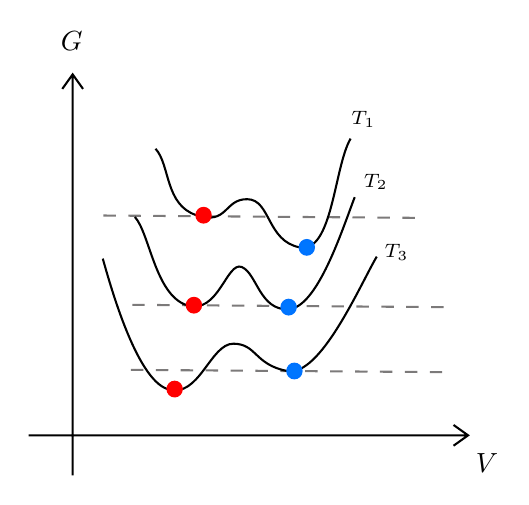
\begin{tikzpicture}[x=0.75pt,y=0.75pt,yscale=-1,xscale=1]
%uncomment if require: \path (0,300); %set diagram left start at 0, and has height of 300

%Straight Lines [id:da3378906674440728] 
\draw [color={rgb, 255:red, 124; green, 122; blue, 122 }  ,draw opacity=1 ] [dash pattern={on 4.5pt off 4.5pt}]  (97,117) -- (247.68,118.12) ;
%Straight Lines [id:da30018625527921405] 
\draw [color={rgb, 255:red, 124; green, 122; blue, 122 }  ,draw opacity=1 ] [dash pattern={on 4.5pt off 4.5pt}]  (110.89,160.03) -- (261.57,161.15) ;
%Straight Lines [id:da4442318288654652] 
\draw [color={rgb, 255:red, 124; green, 122; blue, 122 }  ,draw opacity=1 ] [dash pattern={on 4.5pt off 4.5pt}]  (110.23,191.36) -- (260.91,192.47) ;
%Curve Lines [id:da3655318960367743] 
\draw    (122.1,84.83) .. controls (129.19,92.52) and (126.53,111.86) .. (141.79,116.85) .. controls (157.05,121.85) and (155.06,108.96) .. (166.33,109.13) .. controls (177.61,109.31) and (175.62,129.26) .. (191.54,132.34) .. controls (207.46,135.42) and (208.12,93.49) .. (216.08,79.95) ;
%Curve Lines [id:da5344354372258691] 
\draw    (112.15,117.71) .. controls (119.24,125.39) and (121.89,155.21) .. (137.15,160.2) .. controls (152.4,165.2) and (156.38,138.77) .. (163.68,141.83) .. controls (170.97,144.89) and (172.3,162.94) .. (186.23,162.14) .. controls (200.16,161.33) and (212.1,123.62) .. (218.07,108.15) ;
%Curve Lines [id:da6491468085757098] 
\draw    (96.68,137.77) .. controls (100,149.37) and (112.6,195.62) .. (127.86,200.62) .. controls (143.12,205.61) and (148.42,178.57) .. (159.7,178.75) .. controls (170.97,178.93) and (169.65,188.84) .. (185.57,191.92) .. controls (201.49,194.99) and (220.72,150.34) .. (228.68,136.8) ;
%Shape: Axis 2D [id:dp8880008710750573] 
\draw  (61,222.91) -- (272.68,222.91)(82.17,49) -- (82.17,242.23) (265.68,217.91) -- (272.68,222.91) -- (265.68,227.91) (77.17,56) -- (82.17,49) -- (87.17,56)  ;
%Shape: Ellipse [id:dp31781848539377255] 
\draw  [color={rgb, 255:red, 0; green, 115; blue, 255 }  ,draw opacity=1 ][fill={rgb, 255:red, 0; green, 118; blue, 255 }  ,fill opacity=1 ] (191.54,132.34) .. controls (191.54,130.38) and (193.08,128.8) .. (194.98,128.8) .. controls (196.89,128.8) and (198.43,130.38) .. (198.43,132.34) .. controls (198.43,134.3) and (196.89,135.88) .. (194.98,135.88) .. controls (193.08,135.88) and (191.54,134.3) .. (191.54,132.34) -- cycle ;
%Shape: Ellipse [id:dp6869825687255718] 
\draw  [color={rgb, 255:red, 255; green, 0; blue, 0 }  ,draw opacity=1 ][fill={rgb, 255:red, 255; green, 0; blue, 0 }  ,fill opacity=1 ] (141.79,116.85) .. controls (141.79,114.9) and (143.33,113.31) .. (145.24,113.31) .. controls (147.14,113.31) and (148.68,114.9) .. (148.68,116.85) .. controls (148.68,118.81) and (147.14,120.4) .. (145.24,120.4) .. controls (143.33,120.4) and (141.79,118.81) .. (141.79,116.85) -- cycle ;
%Shape: Ellipse [id:dp1317713936957361] 
\draw  [color={rgb, 255:red, 255; green, 0; blue, 0 }  ,draw opacity=1 ][fill={rgb, 255:red, 255; green, 0; blue, 0 }  ,fill opacity=1 ] (137.15,160.2) .. controls (137.15,158.25) and (138.69,156.66) .. (140.59,156.66) .. controls (142.5,156.66) and (144.04,158.25) .. (144.04,160.2) .. controls (144.04,162.16) and (142.5,163.74) .. (140.59,163.74) .. controls (138.69,163.74) and (137.15,162.16) .. (137.15,160.2) -- cycle ;
%Shape: Ellipse [id:dp88588291364768] 
\draw  [color={rgb, 255:red, 255; green, 0; blue, 0 }  ,draw opacity=1 ][fill={rgb, 255:red, 255; green, 0; blue, 0 }  ,fill opacity=1 ] (127.86,200.62) .. controls (127.86,198.66) and (129.4,197.07) .. (131.31,197.07) .. controls (133.21,197.07) and (134.75,198.66) .. (134.75,200.62) .. controls (134.75,202.57) and (133.21,204.16) .. (131.31,204.16) .. controls (129.4,204.16) and (127.86,202.57) .. (127.86,200.62) -- cycle ;
%Shape: Ellipse [id:dp5820997384354354] 
\draw  [color={rgb, 255:red, 0; green, 115; blue, 255 }  ,draw opacity=1 ][fill={rgb, 255:red, 0; green, 118; blue, 255 }  ,fill opacity=1 ] (182.78,161.14) .. controls (182.78,159.18) and (184.33,157.59) .. (186.23,157.59) .. controls (188.13,157.59) and (189.68,159.18) .. (189.68,161.14) .. controls (189.68,163.09) and (188.13,164.68) .. (186.23,164.68) .. controls (184.33,164.68) and (182.78,163.09) .. (182.78,161.14) -- cycle ;
%Shape: Ellipse [id:dp8696188375819636] 
\draw  [color={rgb, 255:red, 0; green, 115; blue, 255 }  ,draw opacity=1 ][fill={rgb, 255:red, 0; green, 118; blue, 255 }  ,fill opacity=1 ] (185.57,191.92) .. controls (185.57,189.96) and (187.11,188.37) .. (189.01,188.37) .. controls (190.92,188.37) and (192.46,189.96) .. (192.46,191.92) .. controls (192.46,193.87) and (190.92,195.46) .. (189.01,195.46) .. controls (187.11,195.46) and (185.57,193.87) .. (185.57,191.92) -- cycle ;

% Text Node
\draw (75,27) node [anchor=north west][inner sep=0.75pt]   [align=left] {$G$};
% Text Node
\draw (275,230.4) node [anchor=north west][inner sep=0.75pt]    {$V$};
% Text Node
\draw (215,65.4) node [anchor=north west][inner sep=0.75pt]  [font=\scriptsize]  {$T_{1}$};
% Text Node
\draw (221,95.4) node [anchor=north west][inner sep=0.75pt]  [font=\scriptsize]  {$T_{2}$};
% Text Node
\draw (231,129.4) node [anchor=north west][inner sep=0.75pt]  [font=\scriptsize]  {$T_{3}$};


\end{tikzpicture}

    \caption{$G$ vs. $V$ plots for different temperatures.
    \label{fig:water} }
\end{figure}
\noindent
From the previous analysis, we saw that in some interval, we had three values of volume for each pressure (out of which one was unphysical). A physical scenario to imagine is when suppose we have water above its boiling point (so it is in vapour phase). The Gibbs potential has its minima at two volumes as shown in Fig.\ref{fig:water} for curve at $T_1$. The system takes the minima which is lower (the right one).\\[0.2cm] As we decrease the temperature, at some temperature, both the minima become equal, as for $T_2$. This is the \textit{critical temperature}. As temperature is reduced further, the other minima becomes the more stable one. The system was in the right minima which was till now the \textit{stable} one. It still remains in the right one, however, it now becomes \textit{metastable}. In a very small timescale, due to some fluctuations, a \textit{nucleus} of condensed liquid (the stable state) forms which grows rapidly and the entire system undergoes the transition.